\documentclass{nature}

\usepackage{hyperref}
\usepackage{amsmath}
\usepackage{amssymb}
\usepackage{xcolor}
\usepackage{graphicx}

\bibliographystyle{naturemag}

\newcommand{\etaearth}{\eta_\oplus}
\newcommand{\Rpeak}{R_\mathrm{peak}}
\newcommand{\REarth}{R_\oplus}
\newcommand{\Rpl}{R_\mathrm{pl}}

\newcommand{\email}[1]{\href{mailto:#1}{\nolinkurl{#1}}}

\newcommand{\Will}[1]{\textcolor{cyan}{Will: #1}}

\newcommand{\apj}{The Astrophysical Journal}
\newcommand{\apjs}{The Astrophysical Journal Supplement}

\newcommand{\earange}{3.9_{-1.6}^{+2.2}\%}
\newcommand{\rplrange}{3.83_{-0.62}^{+0.76}}
\newcommand{\rpeakrange}{1.25_{-0.17}^{+0.16}}
\newcommand{\corrcoeffrange}{0.334_{-0.053}^{+0.052}}
\newcommand{\fposrange}{7.8_{-1.3}^{+1.4}\%}
\newcommand{\ppeakrange}{0.075_{-0.006}^{+0.007}}
\newcommand{\rhominrange}{5.46^{+0.18}_{-0.18}}
\newcommand{\rhomaxrange}{18.8^{+1.9}_{-1.9}}


\begin{document}
\title{The Occurrence of Earth-Like Planets Around Other Stars}

\author{Will M. Farr$^{1}$, Chris Aldridge$^{1}$, Kirsty Stroud$^{1}$ \& Ilya Mandel$^{1}$}

\maketitle

\begin{affiliations}
\item School of Physics and Astronomy, Univeristy of Birmingham, Birmingham, B15 2TT, United Kingdom
\end{affiliations}

\begin{abstract}
  The quantity $\etaearth$, the number density of planets per star per
  logarithmic planetary radius per logarithmic orbital period at one
  Earth radius and one year periods, describes the occurrence of
  Earth-like extrasolar planets.  Measurement of $\etaearth$ is
  complicated by the difficulty of detecting Earth-like planets in
  Earth-like orbits about Sun-like stars.  Previous
  estimates\cite{2011ApJ...738..151C,2012ApJ...745...20T,2013ApJ...778...53D,2013PNAS..11019273P}
  place $1\% \lesssim \etaearth \lesssim 34\%$.  These works dealt
  with the problem of selection effects in the sample by either
  analyzing a region of the period-radius parameter space where
  observations are complete and extrapolating to $R = \REarth$ and $P
  = 1 \mathrm{yr}$\cite{2011ApJ...738..151C,2012ApJ...745...20T} or
  applying a binned analysis incorporating survey incompletness in the
  period-radius plane\cite{2013ApJ...778...53D,2013PNAS..11019273P}.
  Here we present constraints on $\etaearth$ from a parameterised
  forward model of the (correlated) period-radius distribution and the
  observational selection function in the most recent (Q17) data
  release from the Kepler
  satellite\cite{2010Sci...327..977B,2011ApJ...736...19B,2013ApJS..204...24B}.
  Our data set comprises 181,568 systems observed under the Kepler
  exoplanet observing program, producing 2598 planetary candidates.
  We parameterise the distribution of planetary periods and radii
  using a single, correlated Gaussian component; treat selection
  effects using a parameterised transit detection probability based on
  the measured noise level and stellar properties in the Kepler
  catalog; and include an empirically-parameterised, independent
  component in the planet period-radius distribution to represent
  false-positive planet detections.  Using our model we can
  simultaneously estimate $\etaearth$, place constraints on the planet
  period-radius distribution function, and determine the degree of
  contamination by false-positive candidate indentifications.  We find
  $\etaearth = \earange$ (90\% CL), in agreement with
  Ref.\ \cite{2013PNAS..11019273P}.  However, in contrast to
  Ref.\ \cite{2013PNAS..11019273P}, we can conclude that each star
  hosts $\rplrange$ planets with $P \lesssim 3 \mathrm{yr}$
  and $R \gtrsim 0.2 \REarth$, that the peak of the planet radius
  distribution lies at $\Rpeak = \rpeakrange \REarth$, and
  that $\ln P$ and $\ln R$ are correlated with correlation coefficient
  $r = \corrcoeffrange$ (all 90\% CL).  Our empirical model
  for false-positive contamination is consistent with the dominant
  source being backgroud eclipsing binary
  stars\cite{2013ApJ...766...81F}, with $\fposrange$ (90\%
  CL) of the candidates being false-positives.
\end{abstract}

\begin{figure}
  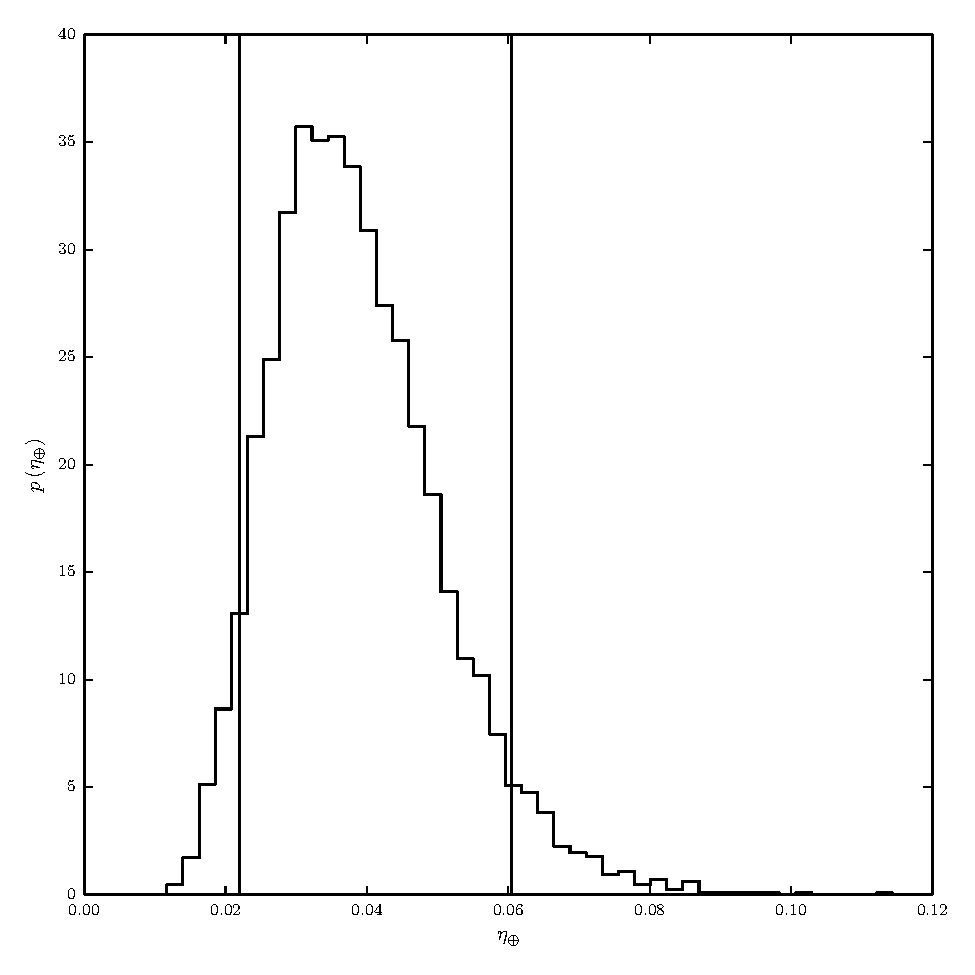
\includegraphics[width=\columnwidth]{eta-earth}
  \caption{\label{fig:eta-earth} \textbf{The posterior on $\etaearth$
      accounting for selection effects and false positives.}  Recall
    that $\etaearth \equiv \left. \frac{dN_\mathrm{pl}}{d\ln P \,d \ln
      R} \right|_{P = 1\mathrm{yr}, R=1\REarth}$.  Vertical lines
    indicate the 90\% credible range.  We find $\etaearth = \earange$,
    in agreement with previous work\cite{2013PNAS..11019273P}.}
\end{figure}

\begin{figure}
  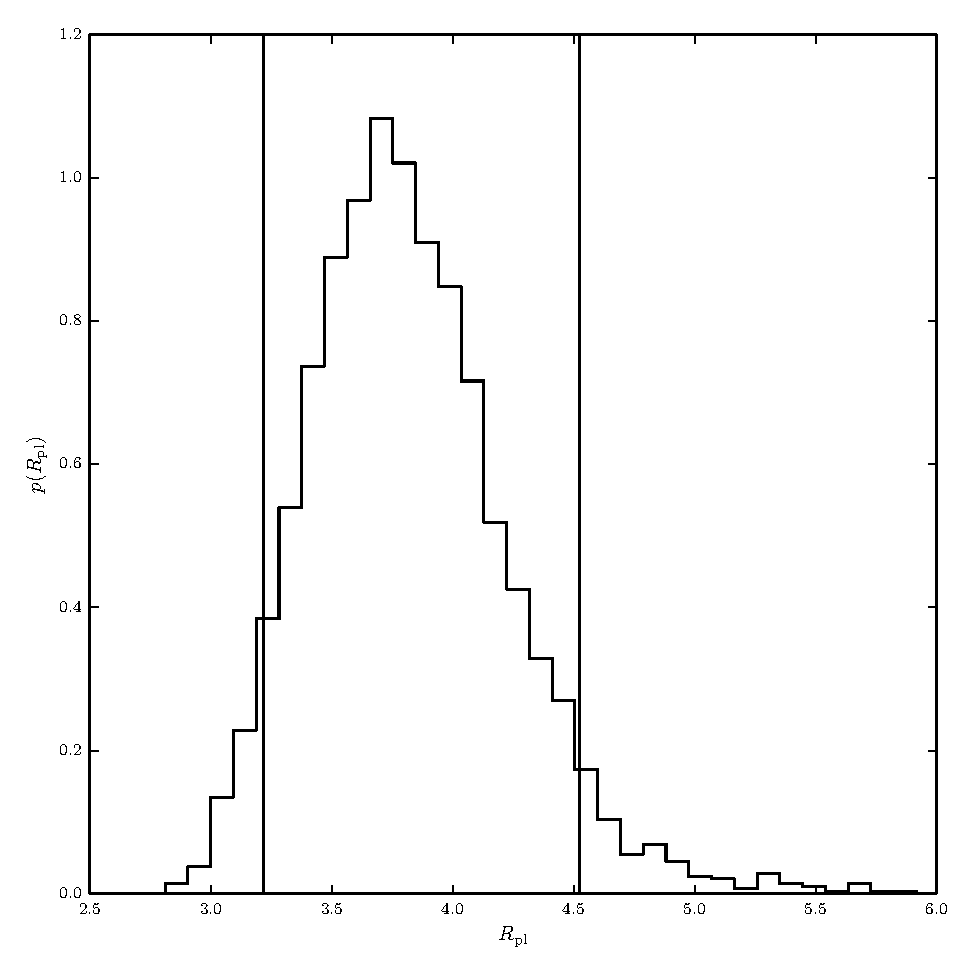
\includegraphics[width=\columnwidth]{npl}
  \caption{\label{fig:npl} \textbf{The posterior on $\Rpl$.}  Recall
    that $\Rpl$ is the number of planets per star.  Vertical lines
    indicate the 90\% credible range.  We find $\Rpl =
    \rplrange$. \Will{CITE/discuss previous work.}}
\end{figure}

\begin{figure}
  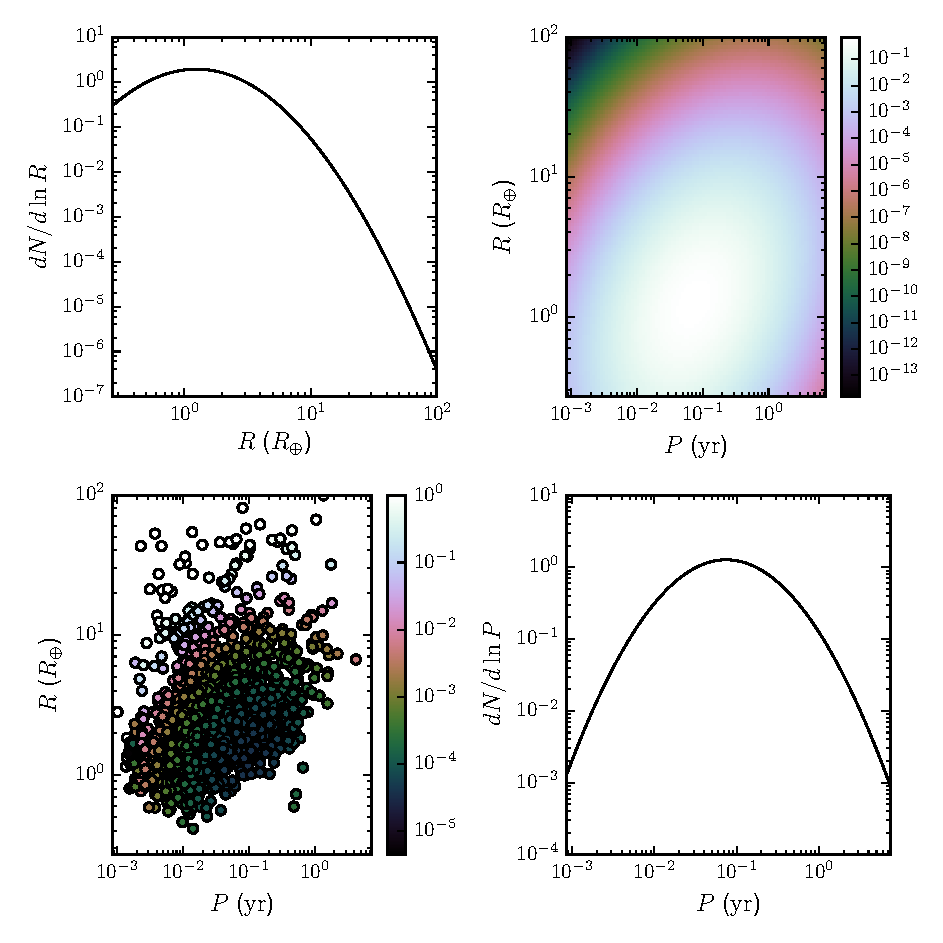
\includegraphics[width=\columnwidth]{foreground-dist}
  \caption{\label{fig:foreground-dist} \textbf{The inferred planet
      period-radius distribution accounting for selection effects and
      false-positives.}  (Upper Left) The planet number density per
    logarithmic planet radius.  The density peaks at $\Rpeak =
    \rpeakrange \REarth$ (90\% CL).  (Upper Right) The planet
    number density in the period-radius plane.  The inferred
    correlation coefficient between $\ln P$ and $\ln R$ is $r =
    \corrcoeffrange$.  (Lower Left) Scatter plot of the radius
    and period of the Kepler planet candidates.  Color indicates the
    posterior false-positive probability for each candidate.  Overall,
    the model prefers a false-positive rate of $\fposrange$
    (90\% CL).  The primary contaminant is probably background
    eclipsing binaries; our contamination rate is consistent with
    previous work\cite{2013ApJ...766...81F}. (Lower Right) The planet
    number density per logarithmic planet period.  The density peaks
    at $P = \ppeakrange \mathrm{yr}$ (90\% CL).}
\end{figure}

\begin{figure}
  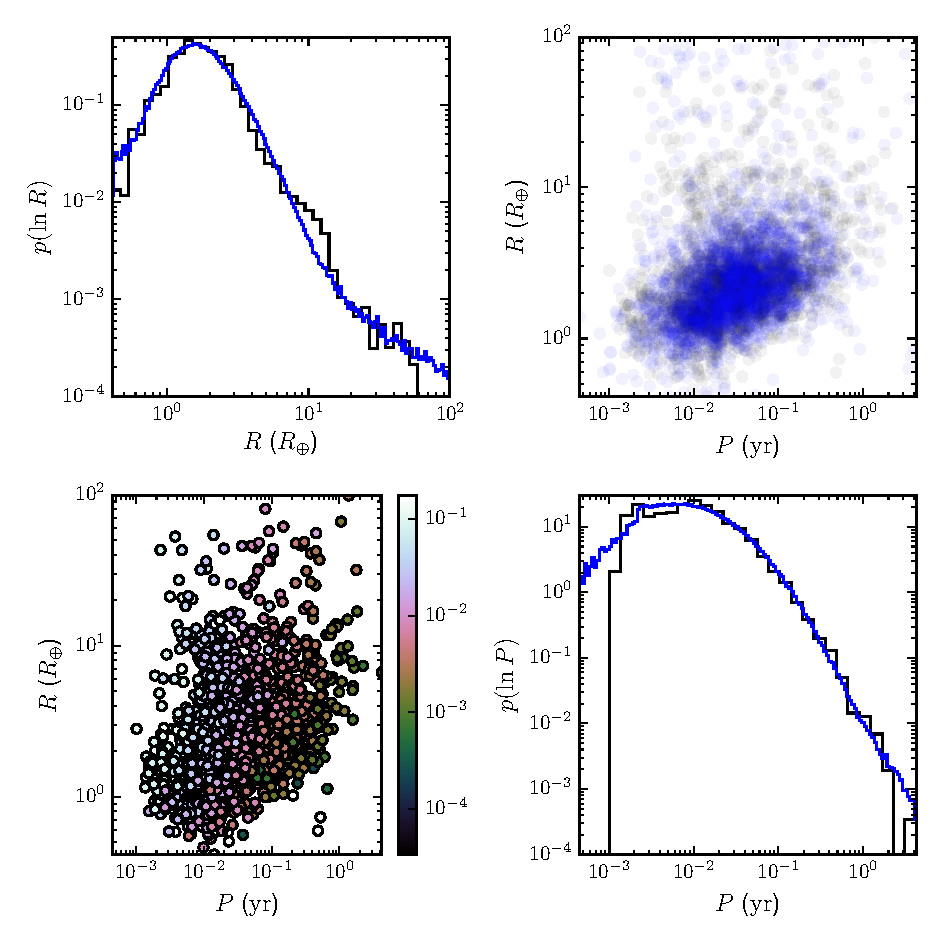
\includegraphics[width=\columnwidth]{selection}
  \caption{\label{fig:selection} \textbf{Comparison of synthetic data
      sets produced from the forward model incorporating selection
      effects with observed candidates.}  (Upper Left) The observed
    (black curve) and synthetic (blue curve; including planets and
    false positives, and using the fitted selection model to
    down-select the candidates from the planet distribution)
    normalised candidate density per logarithmic radius.  Except for a
    discrepancy at $R \simeq 10 \REarth$---associated with hot
    Jupiters, a distinct planetary population\Will{CITE, and
      check}---the model produces a good fit to the observed
    candidates over the range of reported radii.  (Upper Right)
    Scatter plot of the observed candidates (black circles) and a
    posterior-averaged draw of observed candidates from the model
    (blue circles).  (Lower Left) Scatter plot of the observed
    candidates.  Colors indicate the posterior-averaged selection
    probability for each planet about its host star.  Recall that the
    selection probability is treated a product of a geometric factor
    giving the probability of an isotropically-oriented orbit
    producing a transit and a signal-to-noise-ratio-dependent transit
    detection probability.  (Lower Right) The observed (black curve)
    and synthetic (blue curve; including planets and false positives,
    and using the fitted selection model to down-select the candidates
    from the planet distribution) normalised candidate density per
    logarithmic period.  Except for the aforementioned hot Jupiter
    peak at $P \simeq 1 \mathrm{day}$ the model produces a good fit to
    the observed candidates over the range of reported periods.}
\end{figure}

\bibliography{kepler-selection}

\begin{addendum}
\item WMF and IM are supported by a STFC consolidated grant number
  NNNN.  Computations in this work were performed on the University of
  Birmingham's BlueBEAR cluster.  Some/all of the data presented in
  this paper were obtained from the Mikulski Archive for Space
  Telescopes (MAST). STScI is operated by the Association of
  Universities for Research in Astronomy, Inc., under NASA contract
  NAS5-26555. Support for MAST for non-HST data is provided by the
  NASA Office of Space Science via grant NNX13AC07G and by other
  grants and contracts.  This paper includes data collected by the
  Kepler mission. Funding for the Kepler mission is provided by the
  NASA Science Mission directorate.
\item [Author Contributions] All authors assisted in the computational
  modelling, discussed the results, and edited the manuscript.
\item [Reprints] Reprints and permissions information is available at
  \url{www.nature.com/reprints}.
\item[Competing Interests] The authors declare that they have no
  competing financial interests.
\item[Correspondence] Correspondence and requests for materials should
  be addressed to W.M.F.\ (email: \email{w.farr@bham.ac.uk}).
\end{addendum}

\end{document}
